Two thousand points are given on a circle.  Label one of the points 1.  From this point, count 2 points in the clockwise direction and label this point 2.  From the point labeled 2, count 3 points in the clockwise direction and label this point 3.  (See figure.)  Continue this process until the labels $1, 2, 3, \dots, 1993$ are all used.  Some of the points on the circle will have more than one label and some points will not have a label.  What is the smallest integer that labels the same point as 1993?

\begin{center}
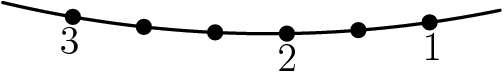
\includegraphics[width = 50.400000000000006mm]{img/fig0.png}
\end{center}